\documentclass[master=eelt,masteroption=ei]{kulemt}
\setup{title={Error bound analysis of sum product networks using posit representation number over FPGA},
  author={Antoine \textsc{Gennart}},
  promotor={Prof.\,dr.\,ir.\ Marian \textsc{Verhelst}},
  assessor={Ir.\, TO FILL},
  assistant={Ir.\ Nimish \textsc{Shah}}}
% The following \setup may be removed entirely if no filing card is wanted
\setup{filingcard,
  translatedtitle=,
  udc=621.3,
  shortabstract={Here comes a very short abstract, containing no more than 500
    words. \LaTeX\ commands can be used here. Blank lines (or the command
% Uncomment the next \setup to generate only the first pages (e.g., if you
% are a Word user.
%\setup{frontpagesonly}
    \texttt{\string\pa r}) are not allowed!
    \endgraf}}
% Uncomment the next line for generating the cover page
%\setup{coverpageonly}

% Choose the main text font (e.g., Latin Modern)
\setup{font=lm}

% If you want to include other LaTeX packages, do it here.
\usepackage{amsmath}
\usepackage{amsfonts}
\usepackage{amssymb}
\usepackage{graphicx}
\usepackage{tikz}
\usepackage{fancyvrb} % for bverbatim
\usepackage{cancel}
\usepackage{subfig}
\usepackage{standalone}
\usepackage{todonotes}
\usepackage[ruled,vlined]{algorithm2e}
\usepackage{algpseudocode}
\usepackage{mdframed}
\usepackage{multirow}


%%
\usepackage{array}
\newcolumntype{L}[1]{>{\raggedright\let\newline\\\arraybackslash\hspace{0pt}}m{#1}}
\newcolumntype{C}[1]{>{\centering\let\newline\\\arraybackslash\hspace{0pt}}m{#1}}
\newcolumntype{R}[1]{>{\raggedleft\let\newline\\\arraybackslash\hspace{0pt}}m{#1}}


%%
\usepackage{pgfplots}
\usepackage{pgfplotstable}
\pgfplotstableset{% global config, for example in the preamble
  every head row/.style={before row=\toprule,after row=\midrule},
  every last row/.style={after row=\bottomrule},
  fixed,precision=2,
}

%%
\usepackage{theorem}
\newtheorem{definition}{Definition}

%%
\usepackage[acronym]{glossaries}
\makeglossaries
\newacronym{Unum}{Unum}{universal number}
\newacronym{spn}{SPN}{sum product network}
\newacronym{hdl}{HDL}{hardware description language}
\newacronym{fpga}{FPGA}{field programable gate array}
\newacronym{ram}{RAM}{random access memory}
\newacronym{cpu}{CPU}{central processing unit}
\newacronym{axi}{AXI}{advanced extensible interface}
\newacronym[firstplural=digital signal processing (DSPs)]{dsp}{DSP}{digital signal processing}
\newacronym{lut}{LUT}{look up table}
\newacronym{jtag}{JTAG}{joint test action group}

\pgfplotsset{compat=1.13}

\usetikzlibrary{positioning}
\usetikzlibrary{shapes,arrows}

% Finally the hyperref package is used for pdf files.
% This can be commented out for printed versions.
\usepackage[pdfusetitle,colorlinks,plainpages=false]{hyperref}

\begin{document}

\begin{preface}
TODODODOD
  I would like to thank everybody who kept me busy the last year,
  especially my promoter and my assistants. I would also like to thank the
  jury for reading the text. My sincere gratitude also goes to my wive and
  the rest of my family.
\end{preface}

\tableofcontents*

\begin{abstract}
\todo[inline]{abstract..}
  The \texttt{abstract} environment contains a more extensive overview of
  the work. But it should be limited to one page.
\end{abstract}

% Now comes the main text
\mainmatter

%!TEX root = ./thesis.tex

\chapter{Introduction}
\label{cha:intro}

This work focus on the implementation of \glspl{spn} in \gls{fpga} using low precision numbers. Two numbers representation are studied: Posit representation, also known as type III \gls{unum} \cite{posit_std} and floating point representation \cite{float_std}. Posit is a quite new standard (2017) and has a lot of advantages compared to floating point such has an increased range of numbers and an increased precision for a large range of values. However, there are some disadvantages to posit, such as the increased hardware size, that justify the fact that it is not a good idea to completely replace floating point by posit for general operations. In this work, we focus on the use of posit for specific use case of \glspl{spn} and try to find out in what cases posit would be preferable to floating point.

Chapter \ref{cha:soa} begins with theory about \gls{spn}. \Glspl{spn} are a new architecture \cite{spns} of deep networks for graphical probabilistic inference. This architecture is designed to make the partition function tractable. Tractable means that it is possible to retrieve the impact of each input feature of the network on the output. Then, low precision arithmetic, namely posit \cite{posit_std} and floating point \cite{float_std} standard are described. Posit and floating point are two number representations as binary string for computer based arithmetic. While floating point is widely used on all electronic devices up to now, posit is a new standard which has a lot of advantages compared to floating point and may be more efficient in a lot of applications. Therefore, this work studies the use of posit in \gls{spn}.

In Chapter \ref{cha:eb}, a model is developed to compute an error bound for posit representation based on the error bound for floating point in \cite{errorbound_float}. Number representation used in this work does not conforms to standard of posit and floating point respectively defined in \cite{posit_std} and \cite{float_std}. Each number representation uses a custom definition of the fields length to minimize the error bound. This error bound represents an upper bound for any set of inputs of the \gls{spn}. As in \cite{errorbound_float}, relative errors are used since values inside a \gls{spn} may be very small and not be efficiently represented by standard number representation such as double floating point.

Then, the development of an hardware implementation of \gls{spn} using custom posit representation is done in Chapter \ref{cha:hard}. It uses a trained \gls{spn} as input and shows how to convert it up to \gls{hdl}. This process is automatized, only some meta parameters should be set to generate a new \gls{spn}. An architecture integrating the \gls{spn} alongside with a control unit and memory is built. Thanks to this architecture, the \gls{spn} can be controlled.

Finally, in Chapter \ref{cha:res} , the results from both Chapter \ref{cha:eb} and \ref{cha:hard} are shown. First the error bound for a large set of \gls{spn} is analyzed. Then, the hardware implementation of a specific \gls{spn} is analyzed and demonstrate the operation of the full design.

%!TEX root = ./thesis.tex

\chapter{State of the art}
\label{cha:soa}

% ==============================================================================
\section{Sum product networks}
% ==============================================================================

\begin{definition}{\Gls{spn}}
A \gls{spn} is a rooted acyclic graph with variables as leaves, sum and product as internal nodes, and weighted edges \cite{spns}.
\end{definition}

\Glspl{spn} allows to represent a probability function by keeping the general conditions that makes this function tractable. Two graphical representations from \cite{spns} are shown in Figure \ref{fig:spn_example}. The leaves of this network are the indicators $X_i$ and $\bar{X_i}$. A \gls{spn} represent the probability $P(X_0, \bar{X_0}, ...,  X_N, \bar{X_N})$.

In order to compute a specific set of probability with the evidence that $X_i=0$, the input of the \gls{spn} $X_i$ must be set to $0$ and the indicator $\bar{X_i}$ must be set to $1$. In order to compute a specific set of probability and marginalize over the variable $X_i$, the indicators $X_i$ and $\bar{X_i}$ must both be set to $1$. In any case, the values of the indicator $X_i$ and $\bar{X_i}$ will both be $0$ at the same time.

\begin{figure}[!ht]
\begin{mdframed}
	\includestandalone[width=0.43\linewidth]{../Images/spn_example1}
	\includestandalone[width=0.56\linewidth]{../Images/spn_example2}
	\caption{Examples of \glspl{spn} from \cite{spns}}
	\label{fig:spn_example}
\end{mdframed}
\end{figure}

\subsection{Properties}

Two properties are interesting for \glspl{spn}: it can be complete and consistent. If an \gls{spn} is complete and consistent, it represent a partition function and can be used to compute all the marginals of this partition function.

\begin{definition}{Complete}
A \gls{spn} is complete iff all children of the same sum node have the same scope. A counter example is shown in Figure \ref{fig:incomplete}.
\end{definition}

\begin{definition}{Consistent}
A \gls{spn} is consistent iff no variable appears negated in one child of a product node and non-negated in another. A counter example is shown in Figure \ref{fig:inconsistent}.
\end{definition}

\begin{figure}[!ht]
\begin{mdframed}
	\centering
	\subfloat[incomplete]{\includestandalone{../Images/incomplete} \label{fig:incomplete}}
	\subfloat[inconsistent]{\includestandalone{../Images/inconsistent} \label{fig:inconsistent}}
\end{mdframed}
\end{figure}


\todo[inline]{Maybe add a real application of \gls{spn} as an example ? To be discussed with Nimish}

% ==============================================================================
\section{Floating point representation}
% ==============================================================================

Floating point representation is the most widely used binary representation of numbers for digital applications. The floating point standard IEEE Std 754-2008 is defined in \cite{float_std}. In this work, we do not use floating point number compatible with this standard. The number of bits for the exponent and the fraction may be optimized for a given application. In addition to this, the sign bit is not used since \glspl{spn} are used to represent probabilities, which are only positive numbers.

% ------------------------------------------------------------------------------
\subsection{Floating point bit-fields}
% ------------------------------------------------------------------------------

The general representation of the fields of the floating point representation are shown in Figure \ref{fig:float_repr}. There is a sign bit (which is removed in this work), a certain number of exponent bits, and a certain number of fraction bits with an implicit leading one. In a given application, the number of exponent and fraction bits are fixed and cannot be modified.

\begin{figure}[!ht]
\begin{mdframed}
	\centering
	\includestandalone[width=\linewidth]{../Images/float_format}
	\caption{Floating point format with sign bit. There are three main field: A sign bit (S), a fixed size exponent, and a fraction.}
	\label{fig:float_repr}
\end{mdframed}
\end{figure}

In order to compute the value represented by a floating point number, the Equation \ref{eq:float_repr} must be used where $exp$ represent the signed value of the exponent field and $b_i$ represent the $i^{th}$ bits of the fraction. Depending on the standard used, the exponent can also be encoded using a unsigned integer and be shifted afterward.

\begin{equation}
x = \xcancel{(-1)^s} \cdot 2^{\text{exp}} \cdot \left( 1 + \sum_{i=1}^{N-1} \text{\textbf{b}}_{N-i} \cdot 2^{-i}\right)
\label{eq:float_repr}
\end{equation}

% ------------------------------------------------------------------------------
\subsection{Floating point operation}
% ------------------------------------------------------------------------------
Addition and multiplication operations are also possible using the floating point operation. They require simple operation such as comparison, and shifting. Addition and multiplication are described in Algorithm \ref{alg:float_add} and \ref{alg:float_mult} respectively.

\begin{algorithm}[H]
\SetAlgoLined
\KwResult{r = a + b}
Compare exponent\;
\eIf{a.exp > b.exp}{
	r.exp = a.exp\;
	f1 = a.frac\;
	f2 = b.frac >> (a.exp - b.exp)\;
}{
	r.exp = b.exp\;
	f1 = a.frac >> (b.exp - a.exp)\;
	f2 = b.frac\;
}
r.frac = f1 + f2\;
\If{overflow(r)}{
	r.frac >> 1\;
	r.exp = r.exp + 1\;
}
Return : r\;
\caption{Floating addition}
\label{alg:float_add}
\end{algorithm}

\begin{algorithm}[H]
\SetAlgoLined
\KwResult{r = a $\cdot$ b}
r.exp = a.exp + b.exp\;
r.frac = a.frac $\cdot$ b.frac\;
Return : r\;
\caption{Floating multiplication}
\label{alg:float_mult}
\end{algorithm}


% ==============================================================================
\section{Posit representation}
% ==============================================================================

Just like floating point representation, posit representation is a method to represent a floating point number using a fixed point number of binary units. It is also know as the type III \gls{Unum} \cite{unum_wiki}.

% ------------------------------------------------------------------------------
\subsection{Posit fields}
% ------------------------------------------------------------------------------

Posit format possesses four fields as shown in Figure \ref{fig:posit_shema}. In this work, the sign bit is not used since posit numbers are used to compute \glspl{spn}, which computes probabilities. Therefore, there are only positive numbers to be represented.

\begin{figure}[!ht]
\begin{mdframed}
\centering
\includestandalone{../Images/posit_format}
\caption{POSIT format with sign bit. There are four main fields: A sign bit (S), a regime (k), an exponent (exp) and a fraction (frac).}
\label{fig:posit_shema}
\end{mdframed}
\end{figure}

The regime field makes the specificity of the posit representation. It is a variable size field using unary encoding. That is: the value of this field can be found by computing the number of consecutive identical bits. It ends with one bit which break the sequence. Therefore, the minimum length for this field is two: either ``b10'' or ``b01''. The maximum length for this field is equal to the number of bits of the posit representation minus one (for the sign bit). A sequence starting with a 1 represent a positive number, and a sequence starting with a 0 represent a negative number. A regime of zero is represented by ``b10''.

The exponent field has a fixed size. If there are not enough number of bits left in the posit representation due to the regime variable size, every unknown bit of this field has a value of ``b0''.

The fraction field has the same meaning as the fraction field of the floating point representation. There is also a implicit leading one in this field. The significand is the term used to described the fraction to which we add the leading one.

Given these four fields, one can compute the value using Equation \ref{eq:posit_eq}. In Figure \ref{fig:posit_shema}, it is mentioned that the combination of the regime and the exponent field form the real exponent. It is the case because we must use both these numbers to compute the exponent which is applied to the significand.


\begin{equation}
x = \xcancel{(-1)^s} \cdot 2^{2\cdot es \cdot \text{\textbf{k}}} \cdot 2^\text{\textbf{exp}} \cdot \left( 1 + \sum_{i=1}^{N-1}  \text{\textbf{b}}_{N-i} \cdot 2^{-i} \right)
\label{eq:posit_eq}
\end{equation}

% ------------------------------------------------------------------------------
\subsection{Posit operations}
% ------------------------------------------------------------------------------
Once decoded, posit numbers can be represented as an exponent and a significand. Therefore, a posit addition or multiplication can be performed using Algorithm \ref{alg:float_add} and \ref{alg:float_mult}. However, a posit encoder and decoder must be used. The pseudo code for the encode and decoder are described in Algorithm \ref{alg:posit_enc} and \ref{alg:posit_dec} respectively.

There are two negative impact for posit numbers. First, because it requires two decoders and one encoders, computation time may be longer. Second, the floating point operation that is performed after decoding the input numbers is also slower than a usual floating point operations since the size of each field (exponent and mantissa) would be bigger than for floating point (given the same number of bits for each representation).

\begin{algorithm}[H]
\SetAlgoLined
\KwResult{exp, frac $\leftarrow$ P}
regime = leading\_zero\_counter(P)\;
exp = (P << abs(regime))[0:es]\;
real\_exp = exp + (regime << es)\;
frac = \{1, P[es+1:]\}\;
return real\_exp, frac\;
\caption{Posit decoder}
\label{alg:posit_dec}
\end{algorithm}

\begin{algorithm}[H]
\SetAlgoLined
\KwResult{P $\leftarrow$ exponent, significand}
regime, exp $\leftarrow$ exponent\;
P $\leftarrow$ encode\_unary(regime)\;
P $\leftarrow$ encode\_binary(exp)\;
P $\leftarrow$ encode\_binary(significand)\;
return P\;
\caption{Posit encoder}
\label{alg:posit_enc}
\end{algorithm}


% \begin{algorithm}
% \caption{Posit addition}
% \begin{algorithmic}[1]
% \item \textbf{Decode both inputs}\;
% exp\_A[log(N)+es:0], sig\_A[N-2-es:0] $\leftarrow$ posit\_A[N-1:0]\;
% exp\_B[log(N)+es:0], sig\_B[N-2-es:0] $\leftarrow$ posit\_B[N-1:0]\;
% \item \textbf{Compute difference of exponent}\;
% exp\_diff = exp\_A - exp\_B\;
% \textbf{IF} (exp\_diff $<$ 0)\;
% \indent \indent exp\_high, sig\_high = exp\_B, sig\_B\;
% \indent \indent exp\_low, sig\_low = exp\_A, sig\_A\;
% \indent \indent exp\_diff\_pos = \textbf{not} exp\_diff\;
% \textbf{Else}\;
% \indent \indent exp\_high, sig\_high = exp\_A, sig\_A\;
% \indent \indent exp\_low, sig\_low = exp\_B, sig\_B\;
% \indent \indent exp\_diff\_pos = \textbf{not} exp\_diff\;
% \item \textbf{Shift the low significand}
% sig\_low\_shift = sig\_low $>>$ exp\_diff\_pos\;
% \item \textbf{Add the significand and check for sig overflow}
% sig\_sum\_tmp = sig\_high + sig\_low\_shift\;
% \textbf{If} (sig\_sum\_tmp overflow)\;
% \indent \indent sig\_sum = sig\_sum\_tmp $>>$ 1\;
% \indent  \indent exp\_sum = exp\_high + 1\;
% \textbf{Else}\;
% \indent \indent sig\_sum = sig\_sum\_tmp\;
% \indent  \indent exp\_sum = exp\_high;\
% \item \textbf{Check for special cases}\;
% \item \textbf{Encode output}\;

% \end{algorithmic}
% \label{alg:posit_add}
% \end{algorithm}



% \begin{algorithm}
% \caption{Posit multiplication}
% \begin{algorithmic}[1]
% \item \textbf{Decode both inputs}\;
% exp\_A[log(N)+es:0], sig\_A[N-2-es:0] $\leftarrow$ posit\_A[N-1:0]\;
% exp\_B[log(N)+es:0], sig\_B[N-2-es:0] $\leftarrow$ posit\_B[N-1:0]\;
% \item \textbf{Compute temporary results}\;
% exp\_res\_tmp[log(N)+1:0] = exp\_A + exp\_B\;
% sig\_res\_tmp = sig\_A * sig\_B\;
% \item \textbf{Manage overflow of significand}\;
% \textbf{If} (sig\_overflow)\;
% \indent \indent exp\_res\_tmp2[log(N)+es+1:0] = exp\_res\_tmp $>>$ 1\;
% \indent \indent sig\_res\_tmp2 = sig\_res\_tmp + 1\;
% \textbf{Else}\;
% \indent \indent exp\_res\_tmp2[log(N)+es+1:0] = exp\_res\_tmp\;
% \indent \indent sig\_res\_tmp2 = sig\_res\_tmp\;
% \item \textbf{Manage min and max values}\;
% \textbf{If} (exponent overflow)\;
% \indent \indent exp\_res = max\_exp\_res\_possible\;
% \textbf{Else If} (exponent underflow)\;
% \indent \indent exp\_res = min\_exp\_res\_possible\;
% \textbf{Else}\;
% \indent \indent exp\_res = exp\_res\_tmp2\;
% \item \textbf{Encode result}\;
% \end{algorithmic}
% \label{alg:posit_mul}
% \end{algorithm}

%!TEX root = ./thesis.tex

\chapter{Error bound}
\label{cha:eb}

In this chapter we described the models of error bound for both posit and floating point representation. An error bound is an estimation of the worst case scenario. That means that there are no errors acutally reported in real cases that are bigger than the computed error bound. All errors are computed in absolute value.

% ==============================================================================
\section{Error bound for Float}
% ==============================================================================
As float is a widely used format, there already exists error bounds for floating point representation in the context of \glspl{spn} \cite{errorbound_float}. It uses a relative error bound instead of an absolute error because absolute error for floating point can be very small and cannot be represented by a standard floating point number while a relative error can be represented using floatng point numbers.

In \cite{errorbound_float}, relative error is defined as follow: Given a number $f$, the encoded using a floating point representation is $\hat{f}$ with an absolute error of $\Delta f$ and a relative error of $\epsilon$ as described in Equation \ref{eq:float_error}.

\begin{equation}
	\tilde{f} = f \pm \Delta f = f \cdot \left(1 \pm \frac{\Delta f}{f} \right) = f \cdot (1 \pm \epsilon)
	\label{eq:float_error}
\end{equation}

For \glspl{spn} applications, errors can occurs in three different cases: While encoding a new number for any litterals or any results of an addition or multiplication, while performing an addition and while performing a multiplication. Note that there is a difference between the error made while performing and encoding an operation.

% ------------------------------------------------------------------------------
\subsection{Encoding error}
% ------------------------------------------------------------------------------

The relative error for a floating point number can be computed based on the fraction size ($fs$) as it is done is Equation \ref{eq:float_err_enc}. As the size of floating point fields are constant, this error is a constant for any value encoded. The only exception we take into account is zero which can be encoded with a relative error equals to zero.

\begin{equation}
	|\epsilon| = \left| \frac{\Delta f}{f} \right| \leq 2^{-(fs+1)} = 2^{-(N-es+1)}
	\label{eq:float_err_enc}
\end{equation}

% ------------------------------------------------------------------------------
\subsection{Addition error}
% ------------------------------------------------------------------------------
Given $\epsilon$, the error of encoding a floating point number, a number $a$ with an accumulated relative error of $\epsilon_a$ and a number $b$ with an accumulated relative error $\epsilon_b$. A new error bound for the result of the addition of $a$ and $b$ can be computed through Equation \ref{eq:float_add_err}.

\begin{align}
\begin{split}
\hat{f} &= (\hat{a} + \hat{b}) \cdot (1 \pm \epsilon)\\
		&= (a \cdot (1 \pm \epsilon_a) + b \cdot (1 \pm \epsilon_b))\cdot (1 \pm \epsilon)\\
		&= (a + b + a \epsilon_a + b \epsilon_b) \cdot (1 \pm \epsilon) \\
		&= (a + b) \cdot \left(1 \pm \frac{a}{a + b} \cdot \epsilon_a \pm \frac{b}{a+b} \cdot \epsilon_b \right) \cdot (1 \pm \epsilon) \\
		&\leq (a+b) \cdot (1 \pm max(\epsilon_a, \epsilon_b)) \cdot (1 \pm \epsilon)\\
(1+\epsilon_f) &= (1 \pm max(\epsilon_a, \epsilon_b)) \cdot (1 \pm \epsilon)
\end{split}
\label{eq:float_add_err}
\end{align}

% ------------------------------------------------------------------------------
\subsection{Multiplication error}
% ------------------------------------------------------------------------------
Given $\epsilon$, the error of encoding a floating point number, a number $a$ with an accumulated relative error of $\epsilon_a$ and a number $b$ with an accumulated relative error $\epsilon_b$. A new error bound for the result of the addition of $a$ and $b$ can be computed through Equation \ref{eq:float_mult_err}.

\begin{align}
\begin{split}
\hat{f} &= \hat{a} \cdot \hat{b} \cdot (1 \pm \epsilon)\\
		&= a \cdot (1 \pm \epsilon_a) \cdot b \cdot (1 \pm \epsilon_b)\\
		&= a \cdot b \cdot (1 \pm \epsilon_a) \cdot (1 \pm \epsilon_b) \cdot (1 \pm \epsilon)\\
(1 \pm \epsilon_f) &= (1 \pm \epsilon_a) \cdot (1 \pm \epsilon_b) \cdot (1 \pm \epsilon)
\end{split}
\label{eq:float_mult_err}
\end{align}

% ==============================================================================
\section{Error bound for Posit}
% ==============================================================================
In this section, it is considered that a posit number has $N$ bits (without sign bit), $rs$ is the regime size (variable), $es$ is the number of exponent bits (fixed) and $ms$ is the number of mantissa bits.

As shown in Equation \ref{eq:rel_err}, the relative error for a posit representation can be expressed using the same method as for floating point (Eq. \ref{eq:float_err_enc}). Again, it is more interesting to compute the relative error since posit representation has a wider range than floating point representation. Therefore an absolute error would not be encodable as a floating point numbers.

\begin{equation}
	\hat{p} = p \pm \Delta p = p \cdot \left(1 \pm \frac{\Delta p}{p}\right) = p \cdot (1 \pm \epsilon)
	\label{eq:rel_err}
\end{equation}

Note that there also exists some reasearch about absolute error for posit representation as it is done in \cite{posit_arithmetic} or \cite{bfp}. These require to use a model with a high precision for very small errors.

% ------------------------------------------------------------------------------
\subsection{Encoding error}
% ------------------------------------------------------------------------------

In the same way as it is done for floating point in Equation \ref{eq:float_err_enc}, the encoding error can be computed on the basis of the fraction size $fs$. For posit representation, the fraction size is not constant and depends on the value of the encoded number.

Given a number which is in the bound of the posit representation, the maximum relative error that could occur is expressed by Equation \ref{eq:posit_enc_error}. This error represent the inability to encode one more fraction bit. The fraction size is represented by $fs$, $rs$ represents the regime size and $es$ the exponent size. $N$ is the number of bits of the posit representation.

\begin{equation}
	|\epsilon| = \left |\frac{\Delta p}{p} \right| \leq 2^{-(fs+1)} = 2^{-(N-min(rs+es, N)+1)}
	\label{eq:posit_enc_error}
\end{equation}


In contrast to floating point, this error highly depends on the number to be represented. It would be minimal for numbers around 1, and it would grows for high numbers and very small numbers (closer to 0) as it is shown in Figure \ref{fig:fp_err_model}. The only exception is zero, which can be encoded with a relative error equals to zero.

% ------------------------------------------------------------------------------
\subsection{Addition and multiplication error}
% ------------------------------------------------------------------------------

given that a relative error has the same definition for posit representation (Eq. \ref{eq:rel_err}) than floating point representation (Eq. \ref{eq:float_err_enc}), addition and multiplication error can be computed using the same formulas than those described for floating point in Equations \ref{eq:float_add_err} and \ref{eq:float_mult_err}.

The difference with floating point is that the actual value of the relative error $\epsilon$ is different given the number that is encoded. A summary of floating point and posit error bound model is shown in Figure \ref{fig:fp_err_model}. This shows that posit representation has a wider range that floating point numbers and that the error bound for posit may vary as a function of the numbers to be represented.

\begin{figure}[!ht]
	\centering
	\includestandalone{../Images/posit_error_model}
	\caption{Summary of the error bound model for positive posit and floating point numbers. The flat area for posit corresponds to numbers that can be encoded using a regime size of 2. For larger (or smaller) numbers, the regime size increases and the error increases as well because there are less bits to encode the fraction. Floating point has a constant relative error bound due to its fixed size fraction field.}
	\label{fig:fp_err_model}
\end{figure}


% ==============================================================================
\section{Error bound for SPNs}
% ==============================================================================

% ------------------------------------------------------------------------------
\subsection{Floating point}
% ------------------------------------------------------------------------------

In order to compute the error bound for a \gls{spn}, the error must be computed for each node and be propagated up to the output. The error bound that is computed must be the worst case scenario. Therefore, there should not be any zero values since that is the only exception that can be encoded with a zero error bound.

By setting all the literals to one, and propagating the error up to the output of the \gls{spn}, we can then compute the error bound of floating point representation for a given network.

In addition to this, an additional computation must be done to ensure that floating point can be used to represent every numbers in the \gls{spn} (even the smallest). Therefore the minimum output of the network must also be computed.

% ------------------------------------------------------------------------------
\subsection{Posit}
% ------------------------------------------------------------------------------
Error bound for posit require more work since the encoding error bound depends on the value which is encoded. Two cases must be taken into account: the maximum value of the \gls{spn}, and the minimum non-zero value of the \gls{spn}. Both of these can be the worst case scenario for a \gls{spn} since that are the values that require the most number of regime bits. Therefore there would be less bits allocated to the fraction and the relative error will be high.

\paragraph{Error for maximum output value}

This error can be computed by setting every input literal to one and propagate the error bounds up to the output as it was done for floating point. However, this error is rarely the biggest error since it is common that the maximum output value of the \gls{spn} is equal to one since it represents a probability\footnote{It is not a mandatory condition. If the maximum output of the \gls{spn} is not equal to one, the we should divide any results by the maximum value to get a probability.}

\paragraph{Error for minimum output value}

The smallest value is more difficult to compute since there are a lot of possible combination of inputs. Therefore, a trick is used to get an approximation of the minimum possible value of the \gls{spn}. This trick consist in setting every literal to one (as for the maximum value), and replacing every SUM node by MIN nodes. In this case, the output of the \gls{spn} may not be a valid set of literals. But the output is smaller or equal to the minimum output for a valid set of literals.

In the end, the posit error bound for an \gls{spn} is the maximum value between the relative error bound computed for maximum output value and minimum output value.
%!TEX root = ./thesis.tex

\chapter{Hardware implementation}
\label{cha:hard}

A hardware implementation consist in a set of file written in \gls{hdl} with constraints associated to these files. First, I describe the hardware implementation of operations on posit numbers, which are the basic building blocks of \glspl{spn}. Then I explain how \glspl{spn} hardware files are generated from a trained \gls{spn} file. Finally, I describe the implementation of the \gls{spn} inside the \gls{fpga} with the complete control scheme. The design is intended to work on a Zed Board.

% ==============================================================================
\section{Posit representation}
% ==============================================================================

In this section, I describe how posit operations are performed in hardware. The general schematic is described in Figure \ref{fig:posit_op}. The floating point operation mentioned here represents the operation described in Algorithm \ref{alg:float_add} and \ref{alg:float_mult}. For a posit operation, the size of each field must be properly computed and is different from a classical floating point operation.

\begin{figure}[!ht]
\begin{mdframed}
	\centering
	\includestandalone[width=\linewidth]{../Images/operator}
	\caption{Illustration for posit operations}
	\label{fig:posit_op}
\end{mdframed}
\end{figure}

% ------------------------------------------------------------------------------
\subsection{Encoder and Decoder}
% ------------------------------------------------------------------------------
As posit representation use variable size fields, an encoder and decoder are required to extract useful information from a raw binary sequence.

The encoder schematized in Figure \ref{fig:enc_mod} is composed of two smaller encoder. A first one which convert an exponent into a regime value and an exponent value. And a second one which take as input the regime, the exponent and the significand to output a posit number. It is in this block that the number are truncated in case of rounding and that information is lost.

The decoder schematized in Figure \ref{fig:dec_mod} is basically the inverse of the encoder except that there is no rounding implemented.

\begin{figure}[!ht]
\begin{mdframed}
	\subfloat[Encoder]{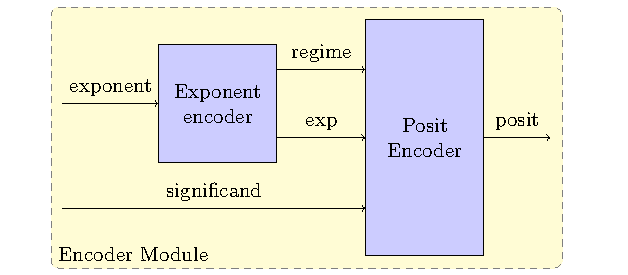
\includegraphics[width=0.49\linewidth]{../Images/encoder_module} \label{fig:enc_mod}}
	\subfloat[Decoder]{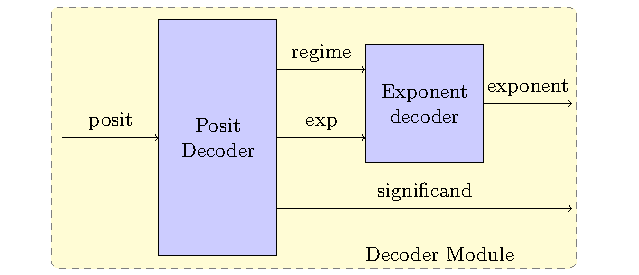
\includegraphics[width=0.49\linewidth]{../Images/decoder_module} \label{fig:dec_mod}}
	\caption{Schematic of encoder and decoder modules}
	\label{fig:enc_dec_mod}
\end{mdframed}
\end{figure}

% ------------------------------------------------------------------------------
\subsection{Adder and multiplier}
% ------------------------------------------------------------------------------
Once posit numbers are decoded into a single exponent and a significand, performing an addition or a multiplication is the same as the application of an addition or a multiplication in the context of floating point numbers as shown in Figure \ref{fig:posit_op}.

From \ref{fig:posit_op}, it is easy to conceive that a posit operation consume more hardware resources than a floating point operation. Note that even the floating point operation performed in the posit operator is bigger than a standard posit operation because the exponent and the significant are of variable size.


% ==============================================================================
\section{Sum product networks}
% ==============================================================================

\Glspl{spn} are built using only adders and multipliers. The challenge of this section is that there exists many different architecture of sum product networks, and that there can be thousands of nodes in a single \gls{spn}. Therefore, we automatized the process of generating a \gls{spn} in \gls{hdl} from a trained one.

% ------------------------------------------------------------------------------
\subsection{PSDD file format}
% ------------------------------------------------------------------------------
In order to generate hardware representation of an \gls{spn}, We choose to use PSDD file format since it was already used by the research group of my daily advisor.

A PSDD file contains three types of nodes: leaf nodes, true nodes and decomposition nodes. Each of these node can be decomposed into a set of wire, sum or product as it is shown in Figure \ref{fig:psdd2spn}.

\begin{figure}[!ht]
\begin{mdframed}
  \centering
  \subfloat[Leaf node]{\includestandalone[scale=0.9]{../Images/literal_node}} \hspace{0.5cm}
  \subfloat[True node]{\includestandalone[scale=0.75]{../Images/true_node}} \hspace{0.5cm}
  \subfloat[Decomposition node]{\includestandalone[scale=0.75]{../Images/decomp_node}}
  \caption{Decomposition of PSDD file into simple arithmetic expression for \gls{spn} format.}
  \label{fig:psdd2spn}
\end{mdframed}
\end{figure}


% ------------------------------------------------------------------------------
\subsection{Pipelining}
% ------------------------------------------------------------------------------
A \gls{spn} can be built using only basic building block such as adder and multiplier, but it would be very slow since the depth of the \gls{spn} can be high. Therefore it is a good idea to pipeline the path from input to output in order to increase the maximum \gls{spn} frequency.

One can not simply add a register at every input or output of every node since some values can skip multiple layers at once. In order to pipeline properly the entire \gls{spn}, the depth of each node must be computed and an appropriate number of register must be set on each path.

\begin{figure}[!ht]
\begin{mdframed}
	\centering
	\includestandalone{../Images/pipeline}
	\caption{Pipelining of SPN. A new register is added every time a path cut a depth level.}
	\label{fig:pip}
\end{mdframed}
\end{figure}

% ==============================================================================
\section{Global system}
% ==============================================================================
Having the hardware code for a \gls{spn} is not sufficient. It is also necessary to be able to control it and request for a specific output given a set of input. In this case, the \gls{spn} is intended to work on a Zed Board \gls{fpga}. In this board, we can have access to a \gls{fpga}, a \gls{ram} and a \gls{cpu} as shown in Figure \ref{fig:glob_workflow}.

\begin{figure}[!ht]
\begin{mdframed}
	\centering
	\includestandalone[width=\linewidth]{../Images/big_picture}
	\caption{Content of zed Board. The \gls{fpga} contains the \gls{spn} and an input module to paralellize the inputs of the \gls{spn}. The embedded operating system launch a software which control the flow of data from the memory to the \gls{spn} and from the \gls{spn} to the memory. Data transfer are performed through \gls{axi} bus}
	\label{fig:glob_workflow}
\end{mdframed}
\end{figure}

% ------------------------------------------------------------------------------
\subsection{FPGA}
% ------------------------------------------------------------------------------
The \gls{fpga} contains the \gls{spn} as well as an input module whose function is to convert a serial input to a parallel output. \Glspl{spn} may have a high number of inputs and the connection from the \gls{ram} to the \gls{fpga} is limited to 32 bits. Therefore this module is required.

The \gls{fpga} is size limited. Not all \gls{spn} will fit inside it. The key limiting factors are the number of slice \glspl{lut} and the number of \glspl{dsp}. A zed Board possesses 53200 slice \glspl{lut} and 220 \glspl{dsp}.

% ------------------------------------------------------------------------------
\subsection{Memory}
% ------------------------------------------------------------------------------
The memory initially contains the software to be executed as well as the set of inputs for which we want to compute the probability.

% ------------------------------------------------------------------------------
\subsection{Control unit}
% ------------------------------------------------------------------------------
The control unit execute the software. It should send data to the \gls{fpga} and receive the output from the \gls{spn}. The maximum frequency of the \gls{fpga} is known by design. Therefore we can just push the data at the best frequency that will not break the \gls{spn} and get the data. Once the data is received, it is sent over stdout which can be accessible through \gls{jtag} to get the data out of the zed board.





%!TEX root = ./thesis.tex

\chapter{Results and experiments}
\label{cha:res}

Two main subjects are introduced in Chapter \ref{cha:eb} and \ref{cha:hard}. In this chapter, results and experiments for these two subjects are shown.


% ==============================================================================
\section{Error bound}
% ==============================================================================

In this section, the error bound for different \glspl{spn} is computed as it was described in \ref{cha:eb}. These error bounds over-estimate the maximum possible relative that is possible to observe in a given \gls{spn}. It may happen that a relatively high error bound is theoretically computed, and that in reality, the error is much smaller or even zero.

It starts by computing the error bound for a relatively small \gls{spn} in order to show exactly how it is computed and how the results can be interpreted. After that, we explore networks for which both floating point and posit representation could be used since the maximum and minimum value in these networks are in range of number format. Then we explore some networks for which only posit representation can be used thanks to its wider range.

The simulation is done using a C++ software available at \url{https://github.com/gennartan/spn_sw}. This software uses double floating point precision as ground truth. It is considered that this format is sufficient to represent error bounds of \gls{spn}. As a reminder, double floating point precision numbers uses 64 bits and 11 bits of exponent. Since double floating point format uses 11 bits of exponents, no more than 11 bits of exponents can be used in the simulation.



% ------------------------------------------------------------------------------
\subsection{Simple example \label{sec:simple_example}}
% ------------------------------------------------------------------------------

Lets start by showing results for an simple example to give an intuition on the results. This examples is shown in Figure \ref{fig:example_03} represents a \gls{spn} with 4 different literals ($1$, $\bar{1}$, $2$, $\bar{2}$) which represents two variables. Each branch has a label for which the error and the possible values are computed in Table \ref{tab:example_03}.

In this example, we use 8-bits posit with 0 bits of exponent, and 8-bits float with 3 bits of exponents. From Table \ref{tab:example_03}, it can be observed that the result has a smaller error bound using floating point representation than using posit representation. This behavior is mainly observed on small network because the values inside the \gls{spn} have a relatively short range. Therefore, encoding the exponent in a fixed size field lead to better results. In general, networks are more likely to have a large range of values and posit will have better results.

\begin{figure}[!ht]
\begin{mdframed}
	\centering
	\includestandalone[scale=0.8]{../Images/spn_example_03}
	\caption{\gls{spn} example with 4 literals (2 variables), 2 sum nodes and 5 product nodes.}
	\label{fig:example_03}
\end{mdframed}
\end{figure}

\begin{table}[!ht]
	\caption{Error analysis for 8 bits posit number with 0 exponent bits and 8 bits float with 3 bits of exponent for the \gls{spn} in Figure \ref{fig:example_03}. Minimum and maximum value represents the minimum (non zero) and maximum value that the node can have. The relative error shows the relative error for posit representation of the minimum value and maximum value. These are the two candidates for worst case of \gls{spn}. The floating point representation only has one column of relative error since it does not depends on the value encoded. The final worst case relative error bound for posit is 0.1672 and for float it is 0.15.}
	\label{tab:example_03}
	\centering
	\begin{tabular}{|c||c|c||c||c|c||c|}
	\hline
		Label & Min value & Max value & rel error Posit & rel error Float\\ \hline
		a & 1 & 1 & $2^{-7}$ & $2^{-6}$ \\ \hline
		b & 0.5 & 0.5 & $2^{-6}$ & $2^{-6}$\\ \hline
		c & 0.5 & 0.5 & 0.0396 & 0.0476 \\ \hline
		d & 0.5 & 1 & 0.0558 & 0.0639 \\ \hline
		e & 0.5 & 1 & 0.0807 & 0.0975 \\ \hline
		f & 1 & 1 & 0.0236 & 0.0476 \\ \hline
		g & 0.25 & 0.5 & 0.1319 & 0.1321 \\ \hline
		h & 0.5 & 0.5 & 0.0559 & 0.0806 \\ \hline \hline
		\textbf{res} & 0.25 & 1 &  \textbf{0.1672} & \textbf{0.150} \\ \hline
	\end{tabular}
\end{table}

% ------------------------------------------------------------------------------
\subsection{Error bound when both posit and float representation are in range}
% ------------------------------------------------------------------------------

Given a number of bits to represent a number, we compute the relative error of floating point and posit representation. Each network was tested with a different number of bits for each representation from the following list : (8, 12, 16, 20, 24, 28). For each number of bits, and each representation, we optimize the exponent size by choosing the value that minimize the relative error from the following list: (0, 2, 3, 4, 6, 8, 10, 11).

In this section, we show only the results when both posit and floating point are in range for the minimum and maximum value of the \gls{spn}. The maximum exponent size which is tested is 11 since it represents the number of exponent bits for double precision floating point numbers which are used by the computer which performed the simulation.

% --------------------------------------
\paragraph{Network 1}
% --------------------------------------

The first network that will be analyzed is the network containing 37460 nodes (28770 products and 8690 sums). For this network, it can be observed that posit representation is better than floating point representation. It can be interpreted by the fact that posit representation with 6 bits of exponent can represent most of the numbers in the \gls{spn} with a minimum regime size\footnote{The minimum regime size is two bits. In this case it can represent a 0 ($b10$) or a -1 ($b10$).}. A higher regime size will be used only in some rare cases.

This show the major limitation of floating point numbers. In order to be able to represent the lower and maximum value of the \gls{spn}, it must have enough exponents bits. Therefore, some exponents bits are useful only in some specific set of literals, and reduce the mean precision of the \gls{spn}.

\begin{table}[!ht]
	\centering
	\caption{Relative error for posit and floating point representation given a \gls{spn} containing 37460 nodes (28770 products, and 8690 sums). The exponent size was optimized to minimize the relative error.}
	\label{tab:net1_res}
	\begin{tabular}{|c||c|c|c||c|c|}
	\hline
		& \multicolumn{2}{c||}{Posit} &  \multicolumn{2}{c|}{Float} \\
	\hline
		\# bits & exp size & rel error & exp size & rel error \\
	\hline
		20 & 6 & 7e-2 & 10 & 3e-1 \\
		24 & 6 & 4e-3 & 10 & 2e-2 \\
		28 & 6 & 3e-4 & 10 & 1e-3 \\
	\hline
	\end{tabular}
\end{table}


% --------------------------------------
\paragraph{Network 2}
% --------------------------------------

The second network contains 3199 nodes (2501 products and 698 sums). It is about 10 times smaller than the previous one. In this case, it is expected that floating point numbers requires less exponent bits are are more competitive.

The results for this network are shown in Table \ref{tab:net2_res}. It can be observed that the worst case of the relative error for posit representation is closer to the relative error of floating point. However, posit is still better than floating point for every number representation.

\begin{table}[!ht]
	\centering
	\caption{Relative error for posit and floating point representation given a \gls{spn} containing 3199 nodes (2501 products and 698 sums). The exponent size was optimized to minimize the relative error.}
	\label{tab:net2_res}
	\begin{tabular}{|c||c|c||	c|c|c|}
	\hline
		& \multicolumn{2}{c||}{Posit} &  \multicolumn{2}{c|}{Float} \\
	\hline
		\# bits & exp size & rel error & exp size & rel error \\
	\hline
		16 & 4 & 1e-1 & 8 & 2e-1 \\
		20 & 4 & 7e-3 & 8 & 1e-2 \\
		24 & 4 & 4e-4 & 8 & 6e-4 \\
		28 & 4 & 3e-5 & 8 & 4e-5 \\
	\hline
	\end{tabular}
\end{table}


From the two examples above, it can be returned that posit representation is better than floating point numbers when both representation are in range of their numbers.



% ------------------------------------------------------------------------------
\subsection{Error bound when posit is in range and floating point representation is not}
% ------------------------------------------------------------------------------
In this section we describe the results when the smallest value of a \gls{spn} can be represented by posit and cannot be represented by a floating point number due to the limited exponent size. The goal is to show that because floating point numbers can not be used in a specific \gls{spn} due to a lack of range, posit can be used and still have an error which is relatively small.

% --------------------------------------
\paragraph{Network 3}
% --------------------------------------

The third network contains 827 nodes (622 products and 205 sums). The results are shown in Table \ref{tab:net3_res}. It can be observed that the error for posit representation is in a reasonable range. For this network, we should use at least 24 bits since the relative error of $0.5$ for 20 bits can be considered as high value.

\begin{table}[!ht]
	\centering
	\caption{Relative error for posit and float representation given a \gls{spn} containing 827 nodes (622 products and 205 sums). The exponent size was optimized to minimize the relative error.}
	\label{tab:net3_res}
	\begin{tabular}{|c||c|c|}
	\hline
		\# bits & exp size & rel error \\
	\hline
		20 & 8 & 5e-1 \\
		24 & 8 & 3e-2 \\
		28 & 8 & 2e-3 \\
	\hline
	\end{tabular}
\end{table}


% ------------------------------------------------------------------------------
\subsection{Error bound when floating point is more suitable than posit}
% ------------------------------------------------------------------------------

In some rare case, floating point representation is more suitable than posit as it was shown in the simple example in Section \ref{sec:simple_example}. The goal here is to prove that even in the worst case \gls{spn}, posit representation remains competitive.

% --------------------------------------
\paragraph{Network 4}
% --------------------------------------

This fourth network contains 7769 nodes (6134 products and 1635 sums). The results are shown in Table \ref{tab:net4_res}. In any case, floating point is more suitable than posit since the relative error is smaller for floating point than for posit. However, they remains very close. In the set of networks that were tested, only a few were more suitable for floating point than posit.

\begin{table}[!ht]
	\centering
	\caption{Relative error for posit and float representation given a \gls{spn} containing 7769 nodes (6134 products and 1635 sums). The exponent size was optimized to minimize the relative error.}
	\label{tab:net4_res}
	\begin{tabular}{|c||c|c||c|c|}
	\hline
		\# bits & exp size & rel error Posit & exp size & rel error Float \\
	\hline
		24 & 8 & 8e-2 & 11 & 5e-2 \\
		28 & 8 & 5e-3 & 11 & 3e-3 \\
	\hline
	\end{tabular}
\end{table}



% ------------------------------------------------------------------------------
\subsection{Analysis of different parameters on a large set of SPNs}
% ------------------------------------------------------------------------------

In this section, only \glspl{spn} which are in range of posit and floating point representation are taken into account.

A first analysis consists in observing the exponent size as a function of then number of bits. Results are shown in Figures \ref{fig:res_mean_es} and \ref{fig:res_mean_es_2}. It can be observed that the optimal exponent size for posit representation is 4 bits less that the optimal exponent size for floating point.

A second analysis consists in observing the mean error as a function of the number of bits. Results are shown in Figures \ref{fig:res_mean_err} and \ref{fig:res_mean_err_2}. The mean relative error is always better for posit than for floating point. However, when using a higher number of bits (28), the error is really close to zero and the actual difference of precision would be very very small.


\begin{figure}[!ht]
\begin{mdframed}
\centering
\subfloat[Mean exponent size]{
	\begin{tikzpicture}
	\begin{axis}[
	    xlabel={Number of bits},
	    ylabel={Mean exponent size},
	    xtick={16, 20, 24, 28},
	    ymin=3.5, ymax=10.5,
	    legend pos=south east,
	    legend entries={Posit, Float},
	    width=0.45\linewidth
	    ]
	  \addplot table [x=nBits,y=esPosit] {test.csv};
	  \addplot table [x=nBits,y=esFloat] {test.csv};
	\end{axis}
	\end{tikzpicture}
	\label{fig:res_mean_es}
}
\subfloat[Mean error]{
	\begin{tikzpicture}
	\begin{axis}[
	    xlabel={Number of bits},
	    ylabel={Mean relative error},
	    xtick={16, 20, 24, 28},
	    ymin=-0.025, ymax=0.25,
	    legend pos=north east,
	    legend entries={Posit, Float},
	    width=0.45\linewidth
	    ]
	  \addplot table [x=nBits,y=minRelErrPosit] {test.csv};
	  \addplot table [x=nBits,y=maxRelErrFloat] {test.csv};
	\end{axis}
	\end{tikzpicture}
	\label{fig:res_mean_err}
}
\caption{Mean exponent size (left) and mean relative error (right) as a function of the number of bits of a large set of \glspl{spn}. This graphic is generated by generating each point with all the \glspl{spn} that are able for this number of bits. This induce a small bias in the results and explain the fact that error bound for 16 bits is smaller than 32 bits (the networks that works for 16 bits usually have a smaller error).}
\label{fig:res_mean}
\end{mdframed}
\end{figure}


\begin{figure}[!ht]
\begin{mdframed}
\centering
\subfloat[Mean exponent size]{
	\begin{tikzpicture}
	\begin{axis}[
	    xlabel={Number of bits},
	    ylabel={Mean exponent size},
	    xtick={16, 20, 24, 28},
	    ymin=3.5, ymax=10.5,
	    legend pos=south east,
	    legend entries={Posit, Float},
	    width=0.45\linewidth
	    ]
	  \addplot table [x=nBits,y=esPosit] {test_2.csv};
	  \addplot table [x=nBits,y=esFloat] {test_2.csv};
	\end{axis}
	\end{tikzpicture}
	\label{fig:res_mean_es_2}
}
\subfloat[Mean error]{
	\begin{tikzpicture}
	\begin{axis}[
	    xlabel={Number of bits},
	    ylabel={Mean relative error},
	    xtick={16, 20, 24, 28},
	    ymin=-0.025, ymax=0.25,
	    legend pos=north east,
	    legend entries={Posit, Float},
	    width=0.45\linewidth
	    ]
	  \addplot table [x=nBits,y=minRelErrPosit] {test_2.csv};
	  \addplot table [x=nBits,y=maxRelErrFloat] {test_2.csv};
	\end{axis}
	\end{tikzpicture}
	\label{fig:res_mean_err_2}
}
\caption{Mean exponent size (left) and mean relative error (right) as a function of the number of bits of a large set of \glspl{spn}. This grahic is generated using all the \glspl{spn} that are in range for 16 bits posit. Therefore the error becomes very small for larger size.}
\label{fig:res_mean_2}
\end{mdframed}
\end{figure}

% ==============================================================================
\section{Hardware implementation}
% ==============================================================================

A complete hardware implementation can be found at \url{https://github.com/gennartan/Arithmetic_circuit_Posit_FPGA}. It contains all the necessary code to implement a \gls{spn} on a \gls{fpga} according to Figure \ref{fig:glob_workflow}.

The parameters to be set are the number of bits, the size of the exponent, the number of bits at the input of the \gls{fpga} (limited to 32), and the number of pipeline stage to be used. The key target of this implementation are the size (the \gls{spn} must fit into the \gls{fpga}) and the speed (it must run as quick as possible). Energy consumption is not optimized in this work.

% ------------------------------------------------------------------------------
\subsection{Posit}
% ------------------------------------------------------------------------------

The properties of posit operators are shown in Table \ref{tab:res_add}. It describes the size of these blocks (in terms of \gls{lut}) and the maximum frequency at which these units can run. Results of this sections are also compared to other working \gls{fpga} implementation of posit. This comparison does not compare two identical things since this work does not take into account the sign bit. Therefore there is more space allocated to the different fields of posit, which have a higher cost in hardware than a sign bit.

\begin{table}[!ht]
\centering
\caption{Size and maximum frequency of posit operators reported by Vivado. This table also introduce the results from \cite{other_fpga} which also implements posit operations under a Zed Board \gls{fpga}.}
	\label{tab:res_add}
	\begin{tabular}{|c||c|c|c||c|c|c|}
	\hline
		& \multicolumn{3}{c||}{New implementation} & \multicolumn{3}{c|}{Literature \cite{other_fpga}} \\ \hline
		N & \#\gls{lut}Add & \#\gls{lut}Mult & f(MHz) & \#\gls{lut} Add & \#\gls{lut}Mult & f(MHz) \\ \hline
		8 & 141 & 170 & 67 & & & \\
		16 & 430 & 310+1\gls{dsp} & 45 & 400 & 220+1\gls{dsp} & 32 \\
		32 & 1100 &  850+4\gls{dsp} & 35 & 950 & 570+4\gls{dsp} & 25 \\ \hline
 	\end{tabular}
\end{table}

% ------------------------------------------------------------------------------
\subsection{SPN}
% ------------------------------------------------------------------------------

In this section, we will show that the hardware implementation can be instanciated for a specific \gls{spn}, and that it can be extented to any network which conforms \glspl{psdd} properties. The chosen \gls{spn} has 67 nodes (50 products and 17 sums). The error bound for this network are shown in Table \ref{tab:nethard_res}. This network was chosen because it fits on the Zed Board and because 16 bits posit numbers have enough precision to represent all the numbers in the \gls{spn}. 16 bits posit is the smallest number of bits that could work with a \gls{spn} of the dataset.

\begin{table}
	\centering
	\caption{Relative error for posit and float representation given a \gls{spn} containing 67 nodes (50 products and 17 sums). The exponent size was optimized to minimize the relative error.}
	\label{tab:nethard_res}
	\begin{tabular}{|c||c|c|c||c|c|}
	\hline
		\# bits & exp size & rel error Posit \\
	\hline
		16 & 4 & 5e-2 \\
		20 & 4 & 3e-3 \\
		24 & 4 & 2e-4 \\
		28 & 4 & 1e-5 \\
	\hline
	\end{tabular}
\end{table}


\paragraph{Hardware properties}

After an optimization using Vivado tool, this network uses 11000 \glspl{lut} and 50 \glspl{dsp} which represents approximately one fourth of the available hardware on this Zed Board. This size cannot be directly computed from Table \ref{tab:res_add} because the tool optimizes the network are remove / reduce the size of nodes which are not completely used. This highly depends on the \gls{spn} architecture and on its weights. Without the tool optimization, the network size would be in the range of 20000 \glspl{lut} and 50 \glspl{dsp}.

The \gls{spn} was generated with a frequency of 100 MHz for the input module and 35MHz for the \gls{spn}. Using these frequences, the global system is limited to a maximum thoughput of 35MHz. However, the actual thoughput of the \gls{spn} is equal 13MHz. This result is much lower that was expected. There are two reasons that explains this lack of efficiency. The first reason is that the clock domain syncer at the output of the input module takes two clocks cycle to transfer a data. Only because of this, the maximum expected throughput fall from 35MHz to 17.5MHz. The second reason is that the software that must send the data to the \gls{fpga} must also get the output data. Therefore it will loose some time when it is not sending inputs to the input module.

\paragraph{Error bound verification}

In order to proove that our design works properly and that the error bound is also correctly computed, we test the \gls{spn} with a bunch of inputs for this network that comes from \cite{dataset} and which were introduced in \cite{dataset_1}, \cite{dataset_2}, \cite{dataset_3} and \cite{dataset_4}. If none of these inputs prove to have a relative error bigger than the error bound it can be considered that both the hardware implementation and the error bound are correcly set.

The maximum relative error computed is $0.747111 \cdot 2^{-5} == 2.33e-2$ which is smaller than the computed error bound ($2.33e-2 \leq 5e-2)$. Therefore we can conclude that this error bound is correctly computed. We also computed the mean relative error through the network in order to know if the error observed on an output is seldom or not. The mean relative error computed is equalt to $0.513 \cdot 2^{-5}$ which is close to the maximum relative error.

\subsection{Futher work}

The hardware implementation works properly and can be easily regenerated for any \gls{spn}. However, some particular cases may require additional work in order to run. In this section I describe the limitations of the current implementation and explain what could be done in order to address these problems.

The current hardware posit implementation is able to work only with three different number of bits: 8, 16 and 32. This is due to the use of a custom module designed to count the number of leading zero (or one). To remedy this problem, this module should be upgraded to be able to count the number of leading zero for any number of bits. This could be done by adding padding to the inputs or by creating a new module for this function.

Posit standard describes a specific rounding method. However, due to the fact that the regime is unary coded, the rouding of a number can lead to a specific case where the regime would gain (or lose) one bit and require speciifc hardware module to handle this. It would reduce speed and increases ressources consumption.

The operations designed for posit are only two inputs operations. In a \gls{spn}, it is common to observe nodes with more than two inputs. A possible upgrade to this could be to create specific n-inputs operators which could perform multiple operations at the same time. In order to implement this, the code that generate the \gls{spn} should be update to handle this.

The output of the input module uses a clock domain syncer to send the data to the \gls{spn}. This clock domain syncer is not efficient and require two \gls{spn} clock cycles. Therefore the effective frequency of the \gls{spn} is divided by two. This could be increased by placing a \gls{fifo} at the output of the input module in the same way that there is a \gls{fifo} at the output of the \gls{fpga}.

The complete design is controlled by a software that runs on the Zed Board. The generation of this software is not automated. Therefore it should be written again for any new \gls{spn}. A process to automatize this task could be performed.

\chapter{Conclusion}
\label{cha:conclusion}


%%% Local Variables:
%%% mode: latex
%%% TeX-master: "thesis"
%%% End:



% \appendixpage*          % if wanted
% \appendix
% \include{app-A}
\clearpage

\printglossary[type=\acronymtype]

% \printglossary

\backmatter
% The bibliography comes after the appendices.
% You can replace the standard "abbrv" bibliography style by another one.

\bibliographystyle{abbrv}
\bibliography{references}

\end{document}

%%% Local Variables:
%%% mode: latex
%%% TeX-master: t
%%% End:



% % A list of figures and tables is optional
% %\listoffigures
% %\listoftables
% % If you only have a few figures and tables you can use the following instead
% \listoffiguresandtables
% % The list of symbols is also optional.
% % This list must be created manually, e.g., as follows:
% \chapter{List of Abbreviations and Symbols}
% \section*{Abbreviations}
% \begin{flushleft}
%   \renewcommand{\arraystretch}{1.1}
%   \begin{tabularx}{\textwidth}{@{}p{12mm}X@{}}
%     LoG   & Laplacian-of-Gaussian \\
%     MSE   & Mean Square error \\
%     PSNR  & Peak Signal-to-Noise ratio \\
%   \end{tabularx}
% \end{flushleft}
% \section*{Symbols}
% \begin{flushleft}
%   \renewcommand{\arraystretch}{1.1}
%   \begin{tabularx}{\textwidth}{@{}p{12mm}X@{}}
%     42    & ``The Answer to the Ultimate Question of Life, the Universe,
%             and Everything'' according to \cite{h2g2} \\
%     $c$   & Speed of light \\
%     $E$   & Energy \\
%     $m$   & Mass \\
%     $\pi$ & The number pi \\
%   \end{tabularx}
% \end{flushleft}
